 
\clearpage
\section{Framework of CO$_2$ flux drivers}
\label{ch:CO2fluxseparation}
\paragraph{PRE-LIMINARY!!! PROBABLY A BAD IDEA!!!}

\paragraph{Purpose of CO$_2$ flux separation}
The previous analysis of thermal, physical and biological controls of the Southern Ocean carbon sink asks for an estimate on the relative contributions of change. As the interconnected processes always influence and change each other directly, a clear and clean separation cannot be taken precision, but rather for an \textit{estimate of the first-order drivers} in CO$_2$ flux. In this chapter, I adapt the CO$_2$ flux diagnostics framework from \cite{Lauderdale2016a} for transient changes, as the heat flux formulation in the existing framework contradicts the logic of the thermal pump.

\subsection{Explanation of the framework and its assumptions}
\cite{Lauderdale2016a} assumes an euphotic zone zonal carbon budget box where at the upper boundary CO$_2$ enters and at the lower boundary biology export production leaves the system. The CO$_2$ flux with the atmosphere is further linearly decomposed into heat flux and fresh water contributions. From knowing the actual CO$_2$ flux, the residual is calculated and attributed to ocean circulation and changes in atmospheric pCO$_2$:

\begin{align*}
\text{CO}_2\text{flux}&= 
\underbrace{   \underbrace{    \gamma_\theta \frac{\overline{ F_{\text{heat}}}_{pi,timmean}}{\rho C_p}}_{\text{climatological heat flux}} +\underbrace{\frac{\text{CO}_{2}\text{flux}}{dpCO_2}\left(pCO_{2,\text{thermal}}-pCO_2\right)}_{\text{transient temperature flux}}}_{\text{temperature flux}} \\
&+ \underbrace{\frac{F_W}{\rho_{fw}}\left( \gamma_S S + \gamma_{A_T} A_T-C_T\right)}_{\text{fresh water flux}} \\ 
&+ \underbrace{\left(\frac{1}{2}\text{calcium export}-\text{organic export}\right)}_{\text{biology}}\\
&+\underbrace{\text{residual}}_{\text{circulation \& pCO2 atmospheric increase}}
\end{align*}

\begin{itemize}
 \item \textbf{Temperature Flux}: The CO$_2$ flux due to temperature is separated into a contribution due to climatological long-term heat flux as in \citep{Lauderdale2016a} and transient contribution for short-term SST changes \citep{Takahashi2002}.

The climatological heat flux contribution is derived from the advection-diffusion formula and assumes a thermal equilibrium, therefore the net air-sea heat flux is a constant mean over the pre-industrial period. $\rho$ is the potential density and $C_p$ the heat capacity for sea-water. The linear solubility coefficients $\gamma_\theta$=8.72 mmol C m$^{-3}$ $^\circ$C$^{-1}$ is empirically diagnosed \citep{Lauderdale2016a}.

The transient temperature flux is calculated based on $pCO_{\text{2,thermal}}$ instead of $pCO_{\text{2}}$ (see section \ref{sec:takahashi}).

\begin{align*}
\text{CO}_2 \text{flux}_{\text{thermal}} &= \text{CO}_2\text{flux}(pCO_{\text{2,thermal}}) - \text{CO}_2\text{flux}(pCO_{\text{2}}) \\
 &= k_w \left( pCO_{\text{2,thermal}}-pCO_{\text{2,atm}} - \left( pCO_{\text{2,ocean}} - pCO_{\text{2,atm}} \right) \right) \\
  &= \frac{\text{CO}_2\text{flux}}{dpCO_2} \left( pCO_{\text{2,thermal}} - pCO_{\text{2,ocean}} \right)  \\ \\
 pCO_{\text{2,thermal}} &= \overline{pCO_2}_{runmean12months} \cdot \exp \left[ 0.0423 ^{\circ}C^{-1}\left( T - \overline{T}_{pi,mean} \right) \right]  
\end{align*}


\item \textbf{Fresh water flux}: The formulation of CO$_2$ flux changes due to freshwater changes remains unchanged. The empirically diagnosed linear solubility coefficients $\gamma_S$=-5.93 mmol C m$^{-3}$ psu$^{-1}$ and $\gamma_{A_T}$=+0.81 mmol C m$^{-3}$ (mmol eq)$^{-1}$ reflect dilution effects: When freshwater is added ($F_W $\textgreater$ 0$), the alkalinity concentration decreases which increases CO$_2$ flux and the DIC ($C_T$) concentration decreases which decreases CO$_2$ flux. Due to opposing signs for alkalinity and DIC, the fresh water CO$_2$ nearly annihilates \citep{Lauderdale2016a}.  

\item \textbf{Biology}: There is a bug-fix impacts of export due to primary production. All particulate matter that sinks below the euphotic zone boundary of 90m is considered to contribute to the biological CO$_2$ flux. The soft-tissue pump takes up DIC and transports it out of euphotic zone by organic matter export and thereby increases CO$_2$ flux, whereas the calcium carbonate counter pump does the same, but decreases alkalinity by two units in the euphotic zone which results in an increase in CO$_2$ flux.

\item \textbf{Residual}: Knowing the total CO$_2$ flux and the processes explained above, I can calculate the residual to attribute changes in circulation, e.g. increased upwelling would supply more DIC to the euphotic zone which would then increase CO$_2$ flux. Comparing to the control simulation, the residual also comprises the CO$_2$ increase due to increase pCO$_{\text{2,atm}}$. [Note: I would really like to separated this! Any idea how?]

\end{itemize}





\begin{figure}[h!]
	\centering
	\includegraphics[scale=.55,trim=5.cm 4.7cm 2.7cm 1.3cm,clip]{co2sep}
	\caption{Schematic illustration of CO$_2$ flux separation after \citep{Lauderdale2016a}; it assumes a well-mixed zonal carbon box of the upper-ocean, where CO$_2$ flux (red) is separated in contributions due to heat flux (orange), freshwater (light blue), climate change (gray), biology (green) and a residual for circulation (dark blue)}	
	\label{fig:CO2flux_separation}
\end{figure}

\vspace{1cm}

This approach assumes: \nopagebreak
\begin{itemize}

\item steady state of $C_{sat}$ over seasonal cycle \citep{Lauderdale2016a}
\item all changes in DIC in the box directly reflect a change 1:1 in CO$_2$ flux
\item no change of pCO$_2$(Alk,DIC) regime, no shift to different part of Deffeyes diagrams
\item linearizations of non-linear processes
\item residual as combined contribution of circulation and CO$_2$ due to atmospheric increase

\end{itemize}









%\begin{figure}[h!]
%	\centering
%	\includegraphics[scale=.7,trim=3.cm 11cm 3cm 4cm,clip]{\memberpositive _positive_trend_8_co2flux_separation.pdf}					\includegraphics[scale=.7,trim=3.cm 11cm 3cm 4cm,clip]{\membernegative _positive_trend_8_co2flux_separation.pdf}
%	\caption{Contribution to CO$_2$ flux trend from (a) negative carbon sink trend and from positive carbon sink trend (b) after separation according to \citep{Lauderdale2016a}; CO$_2$ flux (grey) is separated in contributions due to heat flux (red), freshwater (blue), biology (green) and a residual for circulation (black)}	
%	\label{fig:CO2flux_separation_results}
%\end{figure}

\clearpage

\subsection{Validation of the framework in the pre-industrial control state}
Everything below needs a redo!! Except for figures fig. \ref{fig:CO2flux_separation_control} - \ref{fig:CO2flux_separation_hist-control}


Description (fig. \ref{fig:CO2flux_separation_control})

\begin{figure}[h!]
	\centering
	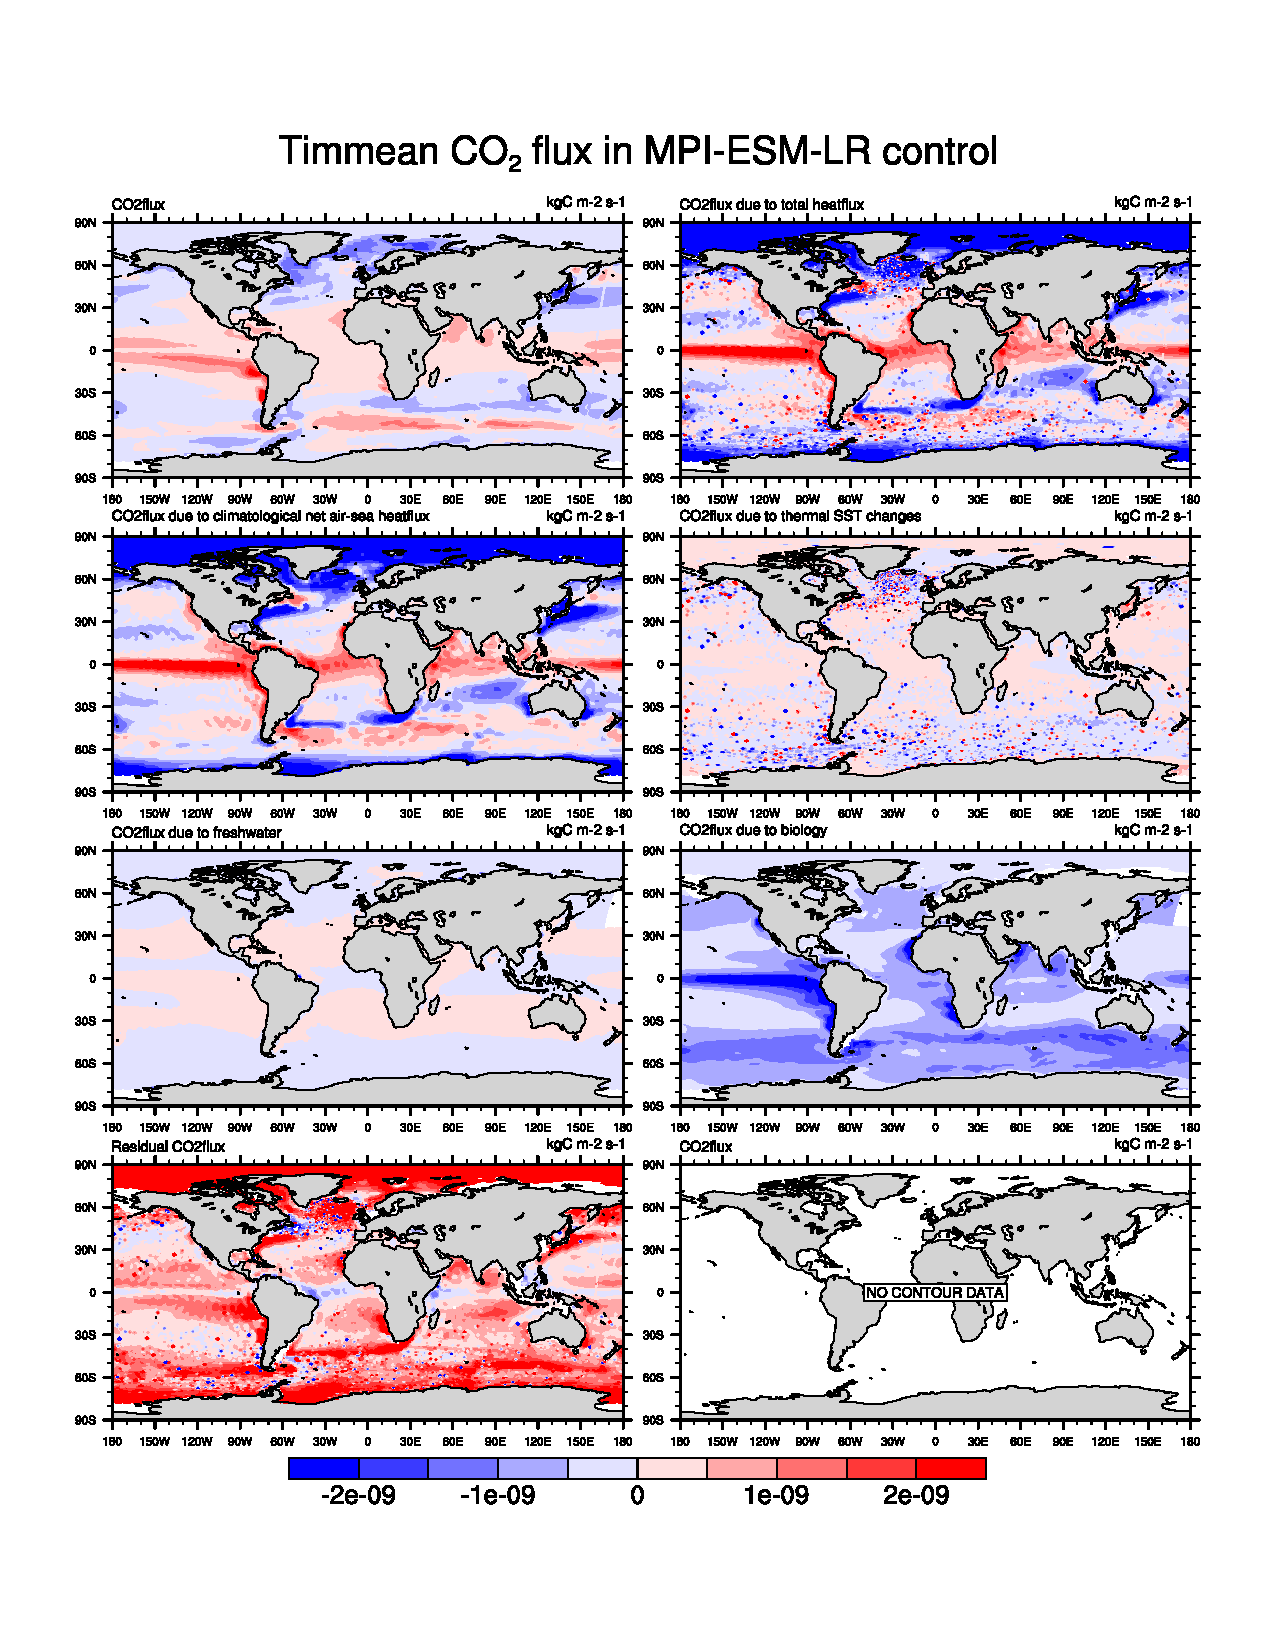
\includegraphics[scale=.8,page=1,trim=1.1cm 2cm 1.1cm 2cm,clip]{method_eval}
	\caption{CO$_2$ flux separation in MPI-ESM LE control}	
	\label{fig:CO2flux_separation_control}
\end{figure}




\subsection{Application of the framework in historical 1980-2004}

Description (fig. \ref{fig:CO2flux_separation_hist})

\begin{figure}[h!]
	\centering
	\includegraphics[scale=.8,page=2,trim=1.1cm 2cm 1.1cm 2cm,clip]{method_eval}
	\caption{CO$_2$ flux separation in MPI-ESM LE historical period 1980 - 2004}	
	\label{fig:CO2flux_separation_hist}
\end{figure}

Changes in climate change (fig. \ref{fig:CO2flux_separation_hist-control})

\begin{figure}[h!]
	\centering
	\includegraphics[scale=.8,page=3,trim=1.1cm 2cm 1.1cm 2cm,clip]{method_eval}
	\caption{Changes in CO$_2$ flux separation in MPI-ESM LE: historical period 1980 - 2004 minus control}	
	\label{fig:CO2flux_separation_hist-control}
\end{figure}

\subsection{Internal Variability in CO$_2$ flux drivers}

timstd map sigma DIV


\subsection{Quantifying drivers in positive and negative CO$_2$ flux trends}

\paragraph{Internal variability in circulation dominates over biology}
By applying the framework from \citep{Lauderdale2016a} to the chosen negative and positive carbon sink trends, I aim to separate the relative contribution of first-order driving mechanisms. 

The mean state CO$_2$ flux due to biology and circulation drive and equalize the carbon system (Table \ref{tab:co2sep_50-60}). Freshwater contribution is negligible, heat flux has a low mean state and climate change predictably has a negative contribution. Looking at internal variability changes importance of contributors: Heat flux, which has a large relative internal variability, becomes more relevant and circulation variations much larger than biology. This suggests that the impact of circulation on the carbon sink is more variable than the impact of biology.

\paragraph{Contributions to positive CO$_2$ flux trend} %m178 cooling
%At 50-60$^\circ$S, the CO$_2$ flux trends in circulation and biology lead equally strong towards increasing carbon sink. The sea-surface warming enhances this slightly as well as the climate change contribution (Table \ref{tab:co2sep_50-60}). %At 40-50$^\circ$S biology increases

figures: SH polar, co2flux, heatflux, bio, residual

\paragraph{Contributions to negative CO$_2$ flux trend} %m143 warming
%At 50-60$^\circ$S, the trends in circulation double the trends of biology. The sea-surface cooling enhances this slightly opposing the small trend in climate change contribution (Table \ref{tab:co2sep_50-60}).


figures: SH polar, co2flux, heatflux, bio, residual

\begin{table}[hbt!]
\begin{tabular}{cccccc}
\multicolumn{6}{c}{50-60$^\circ$S \hspace{1cm} positive carbon sink trend \hspace{.5cm} negative carbon sink trend} \hspace{.5cm} MPI-ESM LE \\
            & PgC/8yrs & \% contribution & PgC/8yrs & \% contribution & PgC/yr\\
\hline \hline %m143			  m178
CO$_2$ flux  & -0.43 & 100 & 0.58 & 100 & -0.05$\pm$0.19\\
\hline
heat flux   &  0.04 & -9 & -0.06 & -11 &  -0.14$\pm$0.05   \\
fresh water &  0.00 & -1 & -0.00 & -1  &  -0.04$\pm$0.00  \\
biology     & -0.17 & 39 & 0.17 & 30  &  -0.76$\pm$0.08  \\
climate change & -0.06 & 13 & -0.01 & -2 &  -0.22$\pm$0.02 \\
circulation & -0.26 & 59 & 0.48 & 60 &  1.11$\pm$0.12  \\
\end{tabular}
\caption{The trends of CO$_2$ flux and its contributions for the zonal band of 50-60$^\circ$S indicate circulation as the most variable contribution}
\label{tab:co2sep_50-60}
\end{table}


\begin{table}[hbt!]
\begin{tabular}{cccccc}
\multicolumn{6}{c}{40-50$^\circ$S \hspace{1cm} positive carbon sink trend \hspace{.5cm} negative carbon sink trend} \hspace{.5cm} MPI-ESM LE\\
            & PgC/8yrs & \% contribution & PgC/8yrs & \% contribution & PgC/yr\\
\hline \hline
CO$_2$ flux  & -0.15 & 100 & -0.03 & 100 &  -0.46$\pm$0.06  \\
\hline
heat flux   &  -0.04 & 25 & 0.12 & -366  &  0.13$\pm$0.06  \\
fresh water & 0.01 & -4 & -0.01 & 27  &  0.02$\pm$0.00  \\
biology     & 0.03 & -19 & -0.07 & 197  &  1.09$\pm$0.03  \\
climate change & -0.03 & 17 & -0.01 & 16  &  -0.23$\pm$0.01  \\
circulation & -0.12 & 83 & -0.08 & 225 &  0.72$\pm$0.06  \\
\end{tabular}
\caption{The trends of CO$_2$ flux and its contributions for the zonal band of 40-50$^\circ$S indicate circulation as the dominant driver over biology and highlights the importance of heat fluxes at lower latitudes }
\label{tab:co2sep_40-50}
\end{table}



%\begin{table}[hbt!]
%\begin{tabular}{ccccc}
%\multicolumn{5}{c}{30-40$^\circ$S \hspace{1cm} positive carbon sink trend \hspace{.5cm} negative carbon sink trend} \\
%            & PgC/8yrs & \% contribution & PgC/8yrs & \% contribution \\
%\hline \hline
%CO$_2$ flux  & -0.06 & 100 & 0.06  & 100\\
%\hline
%heat flux   & -0.05 & 72  & -0.12 & -190 \\
%fresh water & 0.00 & -5   & -0.01 & -12 \\
%biology     & 0.01 & -19  & 0.08 & 126\\
%circulation & -0.03 & 49  & 0.11 & 174\\
%\end{tabular}
%\caption{The trends of CO$_2$ flux and its contributions for the zonal band of 30-40$^\circ$S indicate circulation as the dominant driver over biology and highlights the importance of heat fluxes at lower latitudes }
%\label{tab:co2sep_30-40}

%\end{table}

